\documentclass{article}
\usepackage{tikz}

\begin{document}

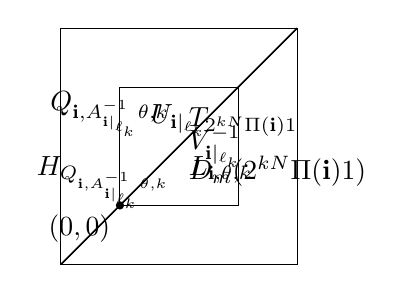
\begin{tikzpicture}[scale=1.5]
    % Draw the large square
    \draw (0,0) -- (2,0) -- (2,2) -- (0,2) -- cycle;
    
    % Draw the smaller square inside the larger one
    \draw (0.5,0.5) -- (1.5,0.5) -- (1.5,1.5) -- (0.5,1.5) -- cycle;
    
    % Label the origin
    \fill (0.5,0.5) circle (1pt);
    \node at (0.5,0.5) [below left] {$(0,0)$};
    
    % Draw the lines connecting the points
    \draw (0,0) -- node[above] {$U_{\mathbf{i}|_{\ell_k}}$} (2,2);
    \draw (0,0) -- node[right] {$V_{\mathbf{i}|_{\ell_k}}^{-1}$} (2,2);
    \draw (0,0) -- node[below right] {$L_{\mathbf{i},\theta,k}$} (2,2);
    \draw (0,0) -- node[below left] {$H_{Q_{\mathbf{i},A_{\mathbf{i}|_{\ell_k}}^{-1}\theta,k}}$} (2,2);
    \draw (0,0) -- node[above left] {$Q_{\mathbf{i},A_{\mathbf{i}|_{\ell_k}}^{-1}\theta,k}$} (2,2);
    \draw (0,0) -- node[above right] {$T_{2^{kN}\Pi(\mathbf{i})\mod 1}$} (2,2);
    \draw (0,0) -- node[below right] {$D_m(2^{kN}\Pi(\mathbf{i})\mod 1)$} (2,2);
\end{tikzpicture}

\end{document}